\documentclass[landscape]{slides}
\usepackage{url}
\usepackage{amsmath}
\usepackage{graphicx}
\usepackage{color}
\usepackage{epic,ecltree}
\usepackage{bar}
\usepackage{eclbip}
\usepackage{multicol}
\usepackage{algorithmic}
\usepackage{algorithm}
\renewcommand{\algorithmicrequire}{\textbf{Input:}}
\renewcommand{\algorithmicensure}{\textbf{Output:}}
\renewcommand{\algorithmiccomment}[1]{// {\em #1}}

\definecolor{darkblue}{rgb}{0,0,0.8}
\definecolor{darkgreen}{rgb}{0,0.8,0}
\definecolor{purple}{rgb}{0.6,0,0.6}
\definecolor{red}{rgb}{1,0,0}

\newcommand{\example}[1]{\textcolor{darkblue}{\rm #1}}
\newcommand{\maths}[1]{\textcolor{purple}{#1}}
\newcommand{\reference}[1]{\vspace{-2mm}\begin{flushright}\textcolor{purple}{\tiny [from #1]}\end{flushright}\vspace{-7mm}}

\begin{document}
\title[Chapter 7: Language Models]{Chapter 7\\[1cm] Language models}
\author[Philipp Koehn]{}
\date{Statistical Machine Translation}

\maketitle

%%%%%%%%%%%%%%%%%%%%%%%%%%%%%%%%%%%%%%%%%%%%%%%%%%%%%%%%%%%%%%%%%%%%%%%%%%%%

\slide{Language models}
\vspace{10mm}
\begin{itemize}
\item {\bf Language models} answer the question:\\[4mm] {\em How likely is a string of English words good English?}
\item Help with reordering
\maths{\begin{equation*}
p_\text{\sc lm}(\text{\example{the house is small}}) > p_\text{\sc lm}(\text{\example{small the is house}})
\end{equation*}}
\item Help with word choice
\maths{\begin{equation*}
p_\text{\sc lm}(\text{\example{I am going home}}) > p_\text{\sc lm}(\text{\example{I am going house}})
\end{equation*}}
\end{itemize}

%%%%%%%%%%%%%%%%%%%%%%%%%%%%%%%%%%%%%%%%%%%%%%%%%%%%%%%%%%%%%%%%%%%%%%%%%%%%

\slide{N-Gram Language Models}
\vspace{10mm}
\begin{itemize}
\item Given: a string of English words \maths{$W = w_1,w_2,w_3,...,w_n$}
\item Question: what is \maths{$p(W)$}?
\item Sparse data: Many good English sentences will not have been seen before
\item[$\rightarrow$] Decomposing \maths{$p(W)$} using the chain rule:
\maths{\begin{equation*}
p(w_1,w_2,w_3,...,w_n) = p(w_1)\;p(w_2|w_1)\;p(w_3|w_1,w_2) ... p(w_n|w_1,w_2,...w_{n-1})
\end{equation*}}
(not much gained yet, \maths{$p(w_n|w_1,w_2,...w_{n-1})$} is equally sparse)
\end{itemize}

%%%%%%%%%%%%%%%%%%%%%%%%%%%%%%%%%%%%%%%%%%%%%%%%%%%%%%%%%%%%%%%%%%%%%%%%%%%%

\slide{Markov Chain}
\vspace{10mm}
\begin{itemize}
\item {\bf Markov assumption}:
\begin{itemize}
\item only previous history matters
\item limited memory: only last $k$ words are included in history \\(older words less relevant)
\item[$\rightarrow$] {\bf $k$th order Markov model}
\end{itemize}
\item For instance 2-gram language model:
\maths{\begin{equation*}
p(w_1,w_2,w_3,...,w_n) \simeq p(w_1)\;p(w_2|w_1)\;p(w_3|w_2) ... p(w_n|w_{n-1})
\end{equation*}}\vspace{-17mm}
\item What is conditioned on, here \maths{$w_{i-1}$} is called the {\bf history}
\end{itemize}

%%%%%%%%%%%%%%%%%%%%%%%%%%%%%%%%%%%%%%%%%%%%%%%%%%%%%%%%%%%%%%%%%%%%%%%%%%%%

\slide{Estimating N-Gram Probabilities}
\vspace{20mm}
\begin{itemize}
\item Maximum likelihood estimation
\maths{\begin{equation*}
p(w_2|w_1) = \frac{\text{count}(w_1,w_2)}{\text{count}(w_1)}
\end{equation*}}\vspace{-17mm}
\item Collect counts over a large text corpus
\item Millions to billions of words are easy to get\\[3mm]
(trillions of English words available on the web)
\end{itemize}

%%%%%%%%%%%%%%%%%%%%%%%%%%%%%%%%%%%%%%%%%%%%%%%%%%%%%%%%%%%%%%%%%%%%%%%%%%%%

\slide{Example: 3-Gram}
\vspace{10mm}
\begin{itemize}
\item Counts for trigrams and estimated word probabilities \vspace{-7mm}
\begin{center}
\begin{tabular}{ccc}

\begin{tabular}{c|c|c}
\multicolumn{3}{c}{\example{the green} (total: 1748)}\\[1mm]
word & c. & prob. \\ \hline \hline
\example{paper} & 801 & 0.458 \\ \hline
\example{group} & 640 & 0.367 \\ \hline
\example{light} & 110 & 0.063 \\ \hline
\example{party} & 27 & 0.015 \\ \hline
\example{ecu} & 21 & 0.012 \\ \hline
\end{tabular}

&

\begin{tabular}{c|c|c}
\multicolumn{3}{c}{\example{the red} (total: 225)}\\[1mm]
word & c. & prob. \\ \hline \hline
\example{cross} & 123 & 0.547 \\ \hline
\example{tape} & 31 & 0.138 \\ \hline
\example{army} & 9 & 0.040 \\ \hline
\example{card} & 7 & 0.031 \\ \hline
\example{,} & 5 & 0.022 \\ \hline
\end{tabular}

&

\begin{tabular}{c|c|c}
\multicolumn{3}{c}{\example{the blue} (total: 54)}\\[1mm]
word & c. & prob. \\ \hline \hline
\example{box} & 16 & 0.296 \\ \hline
\example{.} & 6 & 0.111 \\ \hline
\example{flag} & 6 & 0.111 \\ \hline
\example{,} & 3 & 0.056 \\ \hline
\example{angel} & 3 & 0.056 \\ \hline
\end{tabular}

\end{tabular}
\end{center}
\vspace{5mm}
\begin{itemize}
\item 225 trigrams in the Europarl corpus start with \example{the red}
\item 123 of them end with \example{cross}
\item[$\rightarrow$] maximum likelihood probability is $\frac{123}{225}=0.547$.
\end{itemize}
\end{itemize}

%%%%%%%%%%%%%%%%%%%%%%%%%%%%%%%%%%%%%%%%%%%%%%%%%%%%%%%%%%%%%%%%%%%%%%%%%%%%

\slide{How good is the LM?}
\vspace{20mm}
\begin{itemize}
\item A good model assigns a text of real English \maths{$W$} a high probability
\item This can be also measured with cross entropy:
\maths{\begin{equation*}
H(W) = \frac{1}{n} \log p(W_1^n)
\end{equation*}}
\vspace{-10mm}
\item Or, {\bf perplexity}
\maths{\begin{equation*}
\text{perplexity}(W) = 2^{H(W)}
\end{equation*}}
\end{itemize}

%%%%%%%%%%%%%%%%%%%%%%%%%%%%%%%%%%%%%%%%%%%%%%%%%%%%%%%%%%%%%%%%%%%%%%%%%%%%

\slide{Example: 3-Gram}
\begin{center}
\begin{tabular}{c|c|c} 
prediction & \maths{$p_\text{\sc lm}$} & \maths{-$\log_2 p_\text{\sc lm}$} \\ \hline \hline 
$p_\text{\sc lm}(\text{\example{i}}|\text{\example{\textless /s\textgreater \textless s\textgreater}})$ & 0.109 & 3.197 \\ \hline
$p_\text{\sc lm}(\text{\example{would}}| \text{\example{\textless s\textgreater i}})$      & 0.144 & 2.791 \\ \hline
$p_\text{\sc lm}(\text{\example{like}}|\text{\example{i would}})$    & 0.489 & 1.031\\ \hline
$p_\text{\sc lm}(\text{\example{to}}|\text{\example{would like}})$     & 0.905 & 0.144 \\ \hline
$p_\text{\sc lm}(\text{\example{commend}}|\text{\example{like to}})$   & 0.002 & 8.794 \\ \hline
$p_\text{\sc lm}(\text{\example{the}}|\text{\example{to commend}})$    & 0.472 & 1.084 \\ \hline
$p_\text{\sc lm}(\text{\example{rapporteur}}|\text{\example{commend the}})$& 0.147 & 2.763\\ \hline
$p_\text{\sc lm}(\text{\example{on}}|\text{\example{the rapporteur}})$ & 0.056 & 4.150\\ \hline
$p_\text{\sc lm}(\text{\example{his}}|\text{\example{rapporteur on}})$ & 0.194 & 2.367\\ \hline
$p_\text{\sc lm}(\text{\example{work}}|\text{\example{on his}})$       & 0.089 & 3.498 \\ \hline
$p_\text{\sc lm}(\text{\example{.}}|\text{\example{his work}})$        & 0.290 & 1.785 \\ \hline
$p_\text{\sc lm}(\text{\example{\textless /s\textgreater}}|\text{\example{work .}})$       & 0.99999 & 0.000014 \\ \hline \hline
\multicolumn{2}{r|}{average} & 2.634 \\ 
\end{tabular}
\end{center}

%%%%%%%%%%%%%%%%%%%%%%%%%%%%%%%%%%%%%%%%%%%%%%%%%%%%%%%%%%%%%%%%%%%%%%%%%%%%

\slide{Comparison 1--4-Gram}
\vspace{-1mm}
\begin{center}
\begin{tabular}{c|r|r|r|r} 
word & unigram & bigram & trigram & 4-gram \\ \hline \hline
\example{i}           & 6.684 & 3.197 & 3.197 & 3.197\\ \hline
\example{would}       & 8.342 & 2.884 & 2.791 & 2.791\\ \hline
\example{like}        & 9.129 & 2.026 & 1.031 & 1.290\\ \hline
\example{to}          & 5.081 & 0.402 & 0.144 & 0.113\\ \hline
\example{commend}     &15.487 &12.335 & 8.794 & 8.633\\ \hline
\example{the}         & 3.885 & 1.402 & 1.084 & 0.880\\ \hline
\example{rapporteur}  &10.840 & 7.319 & 2.763 & 2.350\\ \hline
\example{on}          & 6.765 & 4.140 & 4.150 & 1.862\\ \hline
\example{his}         &10.678 & 7.316 & 2.367 & 1.978\\ \hline
\example{work}        & 9.993 & 4.816 & 3.498 & 2.394\\ \hline
\example{.}           & 4.896 & 3.020 & 1.785 & 1.510\\ \hline
\example{\textless /s\textgreater}  & 4.828 & 0.005 & 0.000 & 0.000\\ \hline \hline
average          & 8.051  & 4.072 & 2.634  & 2.251 \\ \hline
perplexity       & 265.136 & 16.817 & 6.206 & 4.758\\
\end{tabular}
\end{center}

%%%%%%%%%%%%%%%%%%%%%%%%%%%%%%%%%%%%%%%%%%%%%%%%%%%%%%%%%%%%%%%%%%%%%%%%%%%%

\slide{Unseen N-Grams}
\vspace{20mm}
\begin{itemize}
\item We have seen \example{i like to} in our corpus
\item We have never seen \example{i like to smooth} in our corpus
\item[$\rightarrow$] \maths{$p(\text{\example{smooth}}|\text{\example{i like to}}) = 0$}
\vspace{10mm}
\item Any sentence that includes \example{i like to smooth} will be assigned probability 0
\end{itemize}

%%%%%%%%%%%%%%%%%%%%%%%%%%%%%%%%%%%%%%%%%%%%%%%%%%%%%%%%%%%%%%%%%%%%%%%%%%%%

\slide{Add-One Smoothing}
\begin{itemize}
\item For all possible n-grams, add the count of one.
\maths{\begin{equation*}
p=\frac{c+1}{n+v}
\end{equation*}}
\vspace{-12mm}
\begin{itemize}
\item \maths{$c$} = count of n-gram in corpus
\item \maths{$n$} = count of history
\item \maths{$v$} = vocabulary size
\end{itemize}
\item But there are many more unseen n-grams than seen n-grams
\item Example: Europarl 2-bigrams:
\begin{itemize}
\item $86,700$ distinct words
\item  $86,700^2 = 7,516,890,000$ possible bigrams
\item but only about $30,000,000$ words (and bigrams) in corpus
\end{itemize}
\end{itemize}

%%%%%%%%%%%%%%%%%%%%%%%%%%%%%%%%%%%%%%%%%%%%%%%%%%%%%%%%%%%%%%%%%%%%%%%%%%%%

\slide{Add-$\alpha$ Smoothing}
\vspace{30mm}
\begin{itemize}
\item Add \maths{$\alpha<1$} to each count
\maths{\begin{equation*}
p=\frac{c+\alpha}{n+\alpha v}
\end{equation*}}
\item What is a good value for  \maths{$\alpha$}?
\item Could be optimized on held-out set
\end{itemize}

%%%%%%%%%%%%%%%%%%%%%%%%%%%%%%%%%%%%%%%%%%%%%%%%%%%%%%%%%%%%%%%%%%%%%%%%%%%%

\slide{Example: 2-Grams in Europarl}
\vspace{5mm}
\begin{center}
\begin{tabular}{|c|c|c|c|} \hline
\bf Count & \multicolumn{2}{c|}{\bf Adjusted count} & \bf Test count \\ \hline
\maths{$c$} & \maths{$(c+1)\frac{n}{n+v^2}$} & \maths{$(c+\alpha)\frac{n}{n+\alpha v^2}$} & \maths{$t_c$}\\ \hline
  0 &  0.00378 &  0.00016 & 0.00016\\ \hline
  1 &  0.00755 &  0.95725 & 0.46235\\ \hline
  2 &  0.01133 &  1.91433 & 1.39946\\ \hline
  3 &  0.01511 &  2.87141 & 2.34307\\ \hline
  4 &  0.01888 &  3.82850 & 3.35202\\ \hline
  5 &  0.02266 &  4.78558 & 4.35234\\ \hline
  6 &  0.02644 &  5.74266 & 5.33762\\ \hline
  8 &  0.03399 &  7.65683 & 7.15074\\ \hline
 10 &  0.04155 &  9.57100 & 9.11927\\ \hline
 20 &  0.07931 & 19.14183 & 18.95948\\ \hline
\end{tabular}
\end{center}
\begin{itemize}\vspace{-2mm}
\item Add-{$\alpha$} smoothing with \maths{$\alpha=0.00017$}\vspace{-8mm}
\item \maths{$t_c$} are average counts of n-grams in test set that occurred \maths{$c$} times in corpus
\end{itemize}

%%%%%%%%%%%%%%%%%%%%%%%%%%%%%%%%%%%%%%%%%%%%%%%%%%%%%%%%%%%%%%%%%%%%%%%%%%%%

\slide{Deleted Estimation}
\begin{itemize}
\item Estimate true counts in held-out data
\begin{itemize}
\item split corpus in two halves: training and held-out
\item counts in training \maths{$C_t(w_1,...,w_n)$}
\item number of ngrams with training count \maths{$r$}: \maths{$N_r$} 
\item total times ngrams of training count \maths{$r$} seen in held-out data: \maths{$T_r$}
\end{itemize}
\item Held-out estimator:
\vspace{-5mm}
\maths{\begin{equation*}
p_h(w_1,...,w_n)=\frac{T_r}{N_rN} \;\; \text{ where $count(w_1,...,w_n)=r$}
\end{equation*}}\vspace{-17mm}
\item Both halves can be switched and results combined
\maths{\begin{equation*}
p_h(w_1,...,w_n)=\frac{T_r^{1}+T_r^{2}}{N(N_r^{1}+N_r^{2})} \;\; \text{where $count(w_1,...,w_n)=r$}\vspace{-17mm}
\end{equation*}}
\end{itemize}

%%%%%%%%%%%%%%%%%%%%%%%%%%%%%%%%%%%%%%%%%%%%%%%%%%%%%%%%%%%%%%%%%%%%%%%%%%%%

\slide{Good-Turing Smoothing}
\vspace{25mm}
\begin{itemize}
\item Adjust actual counts \maths{$r$} to expected counts \maths{$r^*$} with formula
\maths{\begin{equation*}
r^* = (r+1) \frac{N_{r+1}}{N_r}
\end{equation*}}
\begin{itemize}
\item \maths{$N_r$} number of n-grams that occur exactly $r$ times in corpus \vspace{5mm}
\item \maths{$N_0$} total number of n-grams
\end{itemize}
\end{itemize}

%%%%%%%%%%%%%%%%%%%%%%%%%%%%%%%%%%%%%%%%%%%%%%%%%%%%%%%%%%%%%%%%%%%%%%%%%%%%

\slide{Good-Turing for 2-Grams in Europarl}
\vspace{5mm}
\begin{center}
\begin{tabular}{|c|c|c|c|} \hline
\bf Count & \bf Count of counts & \bf Adjusted count & \bf Test count \\ \hline
\maths{$r$} & \maths{$N_r$} & \maths{$r^*$} & \maths{$t$}\\ \hline
  0 & 7,514,941,065 & 0.00015  & 0.00016\\ \hline
  1 & 1,132,844 & 0.46539 & 0.46235\\ \hline
  2 & 263,611 & 1.40679 & 1.39946\\ \hline
  3 & 123,615 & 2.38767 & 2.34307\\ \hline
  4 & 73,788 & 3.33753 & 3.35202\\ \hline
  5 & 49,254 & 4.36967 & 4.35234\\ \hline
  6 & 35,869 & 5.32928 & 5.33762\\ \hline
  8 & 21,693 & 7.43798 & 7.15074\\ \hline
 10 & 14,880 & 9.31304 & 9.11927\\ \hline
 20 & 4,546  & 19.54487 & 18.95948\\ \hline
\end{tabular}

\vspace{5mm}
adjusted count fairly accurate when compared against the test count
\end{center}

%%%%%%%%%%%%%%%%%%%%%%%%%%%%%%%%%%%%%%%%%%%%%%%%%%%%%%%%%%%%%%%%%%%%%%%%%%%%

\slide{Derivation of Good-Turing}
\vspace{25mm}
\begin{itemize}
\item A specific n-gram \maths{$\alpha$} occurs with (unknown) probability \maths{$p$} in the corpus
\item Assumption: all occurrences of an n-gram \maths{$\alpha$} are independent of each other
\item Number of times \maths{$\alpha$} occurs in corpus follows binomial distribution
\maths{\begin{equation*}
p(c(\alpha)=r) = b(r; N,p_i) = \binom{N}{r}p^r(1-p)^{N-r}
\end{equation*}}
\end{itemize}

%%%%%%%%%%%%%%%%%%%%%%%%%%%%%%%%%%%%%%%%%%%%%%%%%%%%%%%%%%%%%%%%%%%%%%%%%%%%

\slide{Derivation of Good-Turing (2)}
\vspace{10mm}
\begin{itemize}
\item Goal of Good-Turing smoothing: compute {\em expected count} \maths{$c^*$}
\item Expected count can be computed with help from binomial distribution:
\maths{\begin{equation*}
\begin{split}
E(c^*(\alpha)) \; &= \sum_{r=0}^N r \; p(c(\alpha)=r)\\
&= \sum_{r=0}^N r \; \binom{N}{r}p^r(1-p)^{N-r}
\end{split}
\end{equation*}}
\vspace{-12mm}
\item Note again: \maths{$p$} is unknown, we cannot actually compute this
\end{itemize}

%%%%%%%%%%%%%%%%%%%%%%%%%%%%%%%%%%%%%%%%%%%%%%%%%%%%%%%%%%%%%%%%%%%%%%%%%%%%

\slide{Derivation of Good-Turing (3)}
\begin{itemize}
\item Definition: expected number of n-grams that occur \maths{$r$} times: \maths{$E_N(N_r)$}
\item We have \maths{$s$} different n-grams in corpus
\vspace{-3mm}
\begin{itemize}
\item let us call them \maths{$\alpha_1,...,\alpha_s$}
\item each occurs with probability \maths{$p_1,...,p_s$}, respectively
\end{itemize}
\item Given the previous formulae, we can compute
\maths{\begin{equation*}
\begin{split}
E_N(N_r) \;&= \sum_{i=1}^s p(c(\alpha_i)=r)\\
&= \sum_{i=1}^s \binom{N}{r}p_i^r(1-p_i)^{N-r}
\end{split}
\end{equation*}}
\vspace{-12mm}
\item Note again: \maths{$p_i$} is unknown, we cannot actually compute this
\end{itemize}

%%%%%%%%%%%%%%%%%%%%%%%%%%%%%%%%%%%%%%%%%%%%%%%%%%%%%%%%%%%%%%%%%%%%%%%%%%%%

\slide{Derivation of Good-Turing (4)}
\begin{itemize}
\item Reflection
\begin{itemize}
\item we derived a formula to compute \maths{$E_N(N_r)$}
\item we have \maths{$N_r$}
\item for small $r$: \maths{$E_N(N_r) \simeq N_r$}
\end{itemize}
\item Ultimate goal compute expected counts \maths{$c^*$}, given actual counts \maths{$c$}
\maths{\begin{equation*}
E(c^*(\alpha)|c(\alpha)=r)
\end{equation*}}
\end{itemize}

%%%%%%%%%%%%%%%%%%%%%%%%%%%%%%%%%%%%%%%%%%%%%%%%%%%%%%%%%%%%%%%%%%%%%%%%%%%%

\slide{Derivation of Good-Turing (5)}
\begin{itemize}
\item For a particular n-gram \maths{$\alpha$}, we know its actual count \maths{$r$}
\item Any of the n-grams \maths{$\alpha_i$} may occur \maths{$r$} times
\item Probability that \maths{$\alpha$} is one specific \maths{$\alpha_i$}
\maths{\begin{equation*}
p(\alpha=\alpha_i|c(\alpha)=r) = \frac{p(c(\alpha_i)=r)}{\sum_{j=1}^s p(c(\alpha_j)=r)}
\end{equation*}}
\vspace{-12mm}
\item Expected count of this n-gram \maths{$\alpha$}
\maths{\begin{equation*}
E(c^*(\alpha)|c(\alpha)=r) = \sum_{i=1}^s N \; p_i \; p(\alpha=\alpha_i|c(\alpha)=r)
\end{equation*}}
\end{itemize}

%%%%%%%%%%%%%%%%%%%%%%%%%%%%%%%%%%%%%%%%%%%%%%%%%%%%%%%%%%%%%%%%%%%%%%%%%%%%

\slide{Derivation of Good-Turing (6)}
\vspace{15mm}
\begin{itemize}
\item Combining the last two equations:
\maths{\begin{equation*}
\begin{split}
E(c^*(\alpha)|c(\alpha)=r) \; &= \sum_{i=1}^s N \; p_i \; \frac{p(c(\alpha_i)=r)}{\sum_{j=1}^s p(c(\alpha_j)=r)}\\
&= \frac{\sum_{i=1}^s N \; p_i \; p(c(\alpha_i)=r)}{\sum_{j=1}^s p(c(\alpha_j)=r)}
\end{split}
\end{equation*}}
\item We will now transform this equation to derive Good-Turing smoothing
\end{itemize}

%%%%%%%%%%%%%%%%%%%%%%%%%%%%%%%%%%%%%%%%%%%%%%%%%%%%%%%%%%%%%%%%%%%%%%%%%%%%

\slide{Derivation of Good-Turing (7)}
\vspace{30mm}
\begin{itemize}
\item Repeat:
\maths{\begin{equation*}
E(c^*(\alpha)|c(\alpha)=r) \; = \frac{\sum_{i=1}^s N \; p_i \; p(c(\alpha_i)=r)}{\sum_{j=1}^s p(c(\alpha_j)=r)}
\end{equation*}}
\vspace{10mm}
\item Denominator is our definition of expected counts \maths{$E_N(N_r)$}
\end{itemize}

%%%%%%%%%%%%%%%%%%%%%%%%%%%%%%%%%%%%%%%%%%%%%%%%%%%%%%%%%%%%%%%%%%%%%%%%%%%%

\slide{Derivation of Good-Turing (8)}
\begin{itemize}
\item Numerator:
\maths{\begin{equation*}
\begin{split}
\sum_{i=1}^s N \; p_i \; p(c(\alpha_i)=r) &\;= \sum_{i=1}^s N \; p_i \; \binom{N}{r}p_i^r(1-p_i)^{N-r} \\
&= N \; \frac{N!}{N-r!r!} p_i^{r+1}(1-p_i)^{N-r} \\
&= N \; \frac{(r+1)}{N+1} \frac{N+1!}{N-r!r+1!} p_i^{r+1}(1-p_i)^{N-r} \\
&= (r+1) \; \frac{N}{N+1} E_{N+1}(N_{r+1}) \\
&\simeq (r+1) \; E_{N+1}(N_{r+1})
\end{split}
\end{equation*}}
\end{itemize} 

%%%%%%%%%%%%%%%%%%%%%%%%%%%%%%%%%%%%%%%%%%%%%%%%%%%%%%%%%%%%%%%%%%%%%%%%%%%%

\slide{Derivation of Good-Turing (9)}
\begin{itemize}
\item Using the simplifications of numerator and denominator:
\maths{\begin{equation*}
\begin{split}
r^* \;&= E(c^*(\alpha)|c(\alpha)=r) \\
&= \frac{(r+1) \; E_{N+1}(N_{r+1})}{E_N(N_r)}\\
&\simeq (r+1) \frac{N_{r+1}}{N_r}
\end{split}
\end{equation*}}
\item QED
\end{itemize}

%%%%%%%%%%%%%%%%%%%%%%%%%%%%%%%%%%%%%%%%%%%%%%%%%%%%%%%%%%%%%%%%%%%%%%%%%%%%

\slide{Back-Off}
\vspace{15mm}
\begin{itemize}
\item In given corpus, we may never observe
\begin{itemize}
\item \example{Scottish beer drinkers}
\item \example{Scottish beer eaters}
\end{itemize}
\item Both have count 0\\[2mm] 
$\rightarrow$ our smoothing methods will assign them same probability
\item Better: backoff to bigrams:
\begin{itemize}
\item \example{beer drinkers}
\item \example{beer eaters}
\end{itemize}
\end{itemize}


%%%%%%%%%%%%%%%%%%%%%%%%%%%%%%%%%%%%%%%%%%%%%%%%%%%%%%%%%%%%%%%%%%%%%%%%%%%%

\slide{Interpolation}
\vspace{15mm}
\begin{itemize}
\item Higher and lower order n-gram models have different strengths and weaknesses
\begin{itemize}
\item high-order n-grams are sensitive to more context, but have sparse counts
\item low-order n-grams consider only very limited context, but have robust counts
\end{itemize}
\item Combine them
\maths{\begin{equation*}
\begin{split}
p_I(w_3|w_1,w_2) = \; & \phantom{\times \;} \lambda_1 \; p_1(w_3) \\
& + \lambda_2 \; p_2(w_3|w_2) \\
& + \lambda_3 \; p_3(w_3|w_1,w_2)
\end{split}
\end{equation*}}
\end{itemize}

%%%%%%%%%%%%%%%%%%%%%%%%%%%%%%%%%%%%%%%%%%%%%%%%%%%%%%%%%%%%%%%%%%%%%%%%%%%%

\slide{Recursive Interpolation}
\vspace{10mm}
\begin{itemize}
\item We can trust some histories \maths{$w_{i-n+1},...,w_{i-1}$} more than others
\item Condition interpolation weights on history: \maths{$\lambda_{w_{i-n+1},...,w_{i-1}}$}
\item Recursive definition of interpolation
\maths{\begin{equation*}
\begin{split}
p^{I}_n(w_i|w_{i-n+1},...,w_{i-1}) = & \; \lambda_{w_{i-n+1},...,w_{i-1}} \;\; p_n(w_i|w_{i-n+1},...,w_{i-1}) \;+\\
	& + \;(1-\lambda_{w_{i-n+1},...,w_{i-1}}) \;\; p^I_{n-1}(w_i|w_{i-n+2},...,w_{i-1})
\end{split}
\end{equation*}}
\end{itemize}

%%%%%%%%%%%%%%%%%%%%%%%%%%%%%%%%%%%%%%%%%%%%%%%%%%%%%%%%%%%%%%%%%%%%%%%%%%%%

\slide{Back-Off}
\vspace{10mm}
\begin{itemize}
\item Trust the highest order language model that contains n-gram
\maths{\begin{equation*}
\begin{split}
p^{BO}_n&(w_i|w_{i-n+1},...,w_{i-1}) =\\
& = 
\begin{cases}
\alpha_n(w_i|w_{i-n+1},...,w_{i-1}) \\
\phantom{--- ---} \text{if count$_n(w_{i-n+1},...,w_i)>0$} \\[2mm]
d_n(w_{i-n+1},...,w_{i-1}) \; p^{BO}_{n-1}(w_i|w_{i-n+2},...,w_{i-1}) \\
\phantom{--- ---}\text{else}
\end{cases}
\end{split}
\end{equation*}}
\vspace{-15mm}
\item Requires 
\begin{itemize}
\item adjusted prediction model \maths{$\alpha_n(w_i|w_{i-n+1},...,w_{i-1})$}
\item discounting function \maths{$d_n(w_1,...,w_{n-1})$}
\end{itemize}
\end{itemize}

%%%%%%%%%%%%%%%%%%%%%%%%%%%%%%%%%%%%%%%%%%%%%%%%%%%%%%%%%%%%%%%%%%%%%%%%%%%%

\slide{Back-Off with Good-Turing Smoothing}
\begin{itemize}
\item Previously, we computed n-gram probabilities based on relative frequency
\vspace{-3mm}
\maths{\begin{equation*}
p(w_2|w_1) = \frac{\text{count}(w_1,w_2)}{\text{count}(w_1)}
\end{equation*}}\vspace{-15mm}
\item Good Turing smoothing adjusts counts \maths{$c$} to expected counts \maths{$c^*$}
\vspace{-3mm}
\maths{\begin{equation*}
\text{count}^*(w_1,w_2) \leq \text{count}(w_1,w_2)
\end{equation*}}\vspace{-15mm}
\item We use these expected counts for the prediction model (but \maths{$0^*$} remains \maths{$0$})
\vspace{-3mm}
\maths{\begin{equation*}
\alpha(w_2|w_1) = \frac{\text{count}^*(w_1,w_2)}{\text{count}(w_1)}
\end{equation*}}\vspace{-15mm}
\item This leaves probability mass for the discounting function
\vspace{-3mm}
\maths{\begin{equation*}
d_2(w_1) = 1 - \sum_{w_2} \alpha(w_2|w_1)\vspace{-20mm}
\end{equation*}}
\end{itemize}

%%%%%%%%%%%%%%%%%%%%%%%%%%%%%%%%%%%%%%%%%%%%%%%%%%%%%%%%%%%%%%%%%%%%%%%%%%%%

\slide{Diversity of Predicted Words}
\vspace{10mm}
\begin{itemize}
\item Consider the bigram histories \example{spite} and \example{constant}
\begin{itemize}
\item both occur 993 times in Europarl corpus
\vspace{3mm}
\item only 9 different words follow \example{spite}\\[1mm]
almost always followed by \example{of} (979 times), due to expression \example{in spite of}
\vspace{3mm}
\item 415 different words follow \example{constant}\\[1mm]
most frequent: \example{and} (42 times), \example{concern} (27 times), \example{pressure} (26 times),\\
but huge tail of singletons: 268 different words
\end{itemize}
\item More likely to see new bigram that starts with \example{constant} than \example{spite}
\item Witten-Bell smoothing considers diversity of predicted words
\end{itemize}

%%%%%%%%%%%%%%%%%%%%%%%%%%%%%%%%%%%%%%%%%%%%%%%%%%%%%%%%%%%%%%%%%%%%%%%%%%%%

\slide{Witten-Bell Smoothing}
\vspace{10mm}
\begin{itemize}
\item Recursive interpolation method
\item Number of possible extensions of a history \maths{$w_1,...,w_{n-1}$} in training data
\maths{\begin{equation*}
N_{1+}(w_1,...,w_{n-1},\bullet) = |\{w_n:c(w_1,...,w_{n-1},w_n)>0\}|
\end{equation*}}
\vspace{-12mm}
\item Lambda parameters
\maths{\begin{equation*}
1-\lambda_{w_1,...,w_{n-1}} = \frac{N_{1+}(w_1,...,w_{n-1},\bullet)}{N_{1+}(w_1,...,w_{n-1},\bullet) + \sum_{w_n} c(w_1,...,w_{n-1},w_n)}
\end{equation*}}
\end{itemize}

%%%%%%%%%%%%%%%%%%%%%%%%%%%%%%%%%%%%%%%%%%%%%%%%%%%%%%%%%%%%%%%%%%%%%%%%%%%%

\slide{Witten-Bell Smoothing: Examples}
\vspace{10mm}
Let us apply this to our two examples:
\maths{\begin{equation*}
\begin{split}
1-\lambda_{\text{\em spite}} \;&= \frac{N_{1+}(\text{\example{spite}},\bullet)}{N_{1+}(\text{\example{spite}},\bullet) + \sum_{w_n} c(\text{\example{spite}},w_n)}\\
&= \frac{9}{9+993} = 0.00898\\[10mm]
1-\lambda_{\text{\em constant}} \;&= \frac{N_{1+}(\text{\example{constant}},\bullet)}{N_{1+}(\text{\example{constant}},\bullet) + \sum_{w_n} c(\text{\example{constant}},w_n)}\\
&= \frac{415}{415+993} = 0.29474
\end{split}
\end{equation*}}


%%%%%%%%%%%%%%%%%%%%%%%%%%%%%%%%%%%%%%%%%%%%%%%%%%%%%%%%%%%%%%%%%%%%%%%%%%%%

\slide{Diversity of Histories}
\vspace{10mm}
\begin{itemize}
\item Consider the word \example{York}
\begin{itemize} 
\item fairly frequent word in Europarl corpus, occurs 477 times 
\item as frequent as \example{foods}, \example{indicates} and \example{providers}
\item[$\rightarrow$] in unigram language model: a respectable probability
\end{itemize}
\item However, it almost always directly follows \example{New} (473 times)
\item Recall: unigram model only used, if the bigram model inconclusive
\begin{itemize}
\item \example{York} unlikely second word in unseen bigram
\item in back-off unigram model, \example{York} should have low probability
\end{itemize}
\end{itemize}

%%%%%%%%%%%%%%%%%%%%%%%%%%%%%%%%%%%%%%%%%%%%%%%%%%%%%%%%%%%%%%%%%%%%%%%%%%%%

\slide{Kneser-Ney Smoothing}
\begin{itemize}
\item Kneser-Ney smoothing takes diversity of histories into account
\item Count of histories for a word
\maths{\begin{equation*}
N_{1+}(\bullet w) \;= |\{ w_i:c(w_i,w)>0 \}|\\
\end{equation*}}
\vspace{-13mm}
\item Recall: maximum likelihood estimation of unigram language model
\maths{\begin{equation*}
p_{ML}(w) = \frac{c(w)}{\sum_i c(w_i)}
\end{equation*}}
\vspace{-13mm}
\item In Kneser-Ney smoothing, replace raw counts with count of histories
\maths{\begin{equation*}
p_{KN}(w) = \frac{N_{1+}(\bullet w)}{\sum_{w_i} N_{1+}(\bullet w_i)}\vspace{-20mm}
\end{equation*}}
\end{itemize}


%%%%%%%%%%%%%%%%%%%%%%%%%%%%%%%%%%%%%%%%%%%%%%%%%%%%%%%%%%%%%%%%%%%%%%%%%%%%

\slide{Modified Kneser-Ney Smoothing}
\begin{itemize}
\item Based on interpolation
\maths{\begin{equation*}
\begin{split}
p^{BO}_n&(w_i|w_{i-n+1},...,w_{i-1}) =\\
& = 
\begin{cases}
\alpha_n(w_i|w_{i-n+1},...,w_{i-1}) \\
\phantom{--- ---} \text{if count$_n(w_{i-n+1},...,w_i)>0$} \\[2mm]
d_n(w_{i-n+1},...,w_{i-1}) \; p^{BO}_{n-1}(w_i|w_{i-n+2},...,w_{i-1}) \\
\phantom{--- ---}\text{else}
\end{cases}
\end{split}
\end{equation*}}
\vspace{-15mm}
\item Requires 
\begin{itemize}
\item adjusted prediction model \maths{$\alpha_n(w_i|w_{i-n+1},...,w_{i-1})$}
\item discounting function \maths{$d_n(w_1,...,w_{n-1})$}
\end{itemize}
\end{itemize}

%%%%%%%%%%%%%%%%%%%%%%%%%%%%%%%%%%%%%%%%%%%%%%%%%%%%%%%%%%%%%%%%%%%%%%%%%%%%

\slide{Formula for $\alpha$ for Highest Order N-Gram Model}
\begin{itemize}
\item Absolute discounting: subtract a fixed \maths{$D$} from all non-zero counts
\maths{\begin{equation*}
\alpha(w_n|w_1,...,w_{n-1}) = \frac{c(w_1,...,w_n)-D}{\sum_{w} c(w_1,...,w_{n-1},w)}
\end{equation*}}
\item Refinement: three different discount values
\maths{\begin{equation*}
D(c) = 
\begin{cases}
D_1 & \text{if} \; c=1\\
D_2 & \text{if} \; c=2\\
D_{3+} & \text{if} \; c \ge 3
\end{cases}
\end{equation*}}
\end{itemize}

%%%%%%%%%%%%%%%%%%%%%%%%%%%%%%%%%%%%%%%%%%%%%%%%%%%%%%%%%%%%%%%%%%%%%%%%%%%%

\slide{Discount Parameters}
\begin{itemize}
\item Optimal discounting parameters $D_1,D_2,D_{3+}$ can be computed quite easily
\maths{\begin{equation*}
\begin{split}
Y \;&= \frac{N_1}{N_1 + 2 N_2}\\
D_1 \;&= 1-2Y\frac{N_2}{N_1}\\
D_2 \;&= 2-3Y\frac{N_3}{N_2}\\
D_{3+} \;&= 3-4Y\frac{N_4}{N_3}
\end{split}
\label{eqn:lm:modified-kneser-ney-absolute-discounts}
\end{equation*}}
\vspace{-12mm}
\item Values \maths{$N_c$} are the counts of n-grams with exactly count \maths{$c$}
\end{itemize}

%%%%%%%%%%%%%%%%%%%%%%%%%%%%%%%%%%%%%%%%%%%%%%%%%%%%%%%%%%%%%%%%%%%%%%%%%%%%

\slide{Formula for $d$ for Highest Order N-Gram Model}
\vspace{15mm}
\begin{itemize}
\item Probability mass set aside from seen events
\maths{\begin{equation*}
d(w_1,...,w_{n-1}) = \frac{\sum_{i\in\{1,2,3+\}}  D_i N_i(w_1,...,w_{n-1}\bullet)}{\sum_{w_n} c(w_1,...,w_n)}
\end{equation*}}
\item \maths{$N_i$} for \maths{$i\in\{1,2,3+\}$} are computed based on the count of extensions of a history \maths{$w_1,...,w_{n-1}$} with count 1, 2, and 3 or more, respectively.
\item Similar to Witten-Bell smoothing
\end{itemize}

%%%%%%%%%%%%%%%%%%%%%%%%%%%%%%%%%%%%%%%%%%%%%%%%%%%%%%%%%%%%%%%%%%%%%%%%%%%%

\slide{Formula for $\alpha$ for Lower Order N-Gram Models}
\vspace{15mm}
\begin{itemize}
\item Recall: base on count of histories $N_{1+}(\bullet w)$ in which word may appear, not raw counts.
\maths{\begin{equation*}
\alpha(w_n|w_1,...,w_{n-1}) = \frac{N_{1+}(\bullet w_1,...,w_n)-D}{\sum_{w} N_{1+}(\bullet w_1,...,w_{n-1},w)}
\end{equation*}}
\item Again, three different values for \maths{$D$} (\maths{$D_1$}, \maths{$D_2$}, \maths{$D_{3+}$}), based on the count of the history \maths{$w_1,...,w_{n-1}$}
\end{itemize}

%%%%%%%%%%%%%%%%%%%%%%%%%%%%%%%%%%%%%%%%%%%%%%%%%%%%%%%%%%%%%%%%%%%%%%%%%%%%

\slide{Formula for $d$ for Lower Order N-Gram Models}
\vspace{35mm}
\begin{itemize}
\item Probability mass set aside available for the \maths{$d$} function
\maths{\begin{equation*}
d(w_1,...,w_{n-1}) = \frac{\sum_{i\in\{1,2,3+\}}  D_i N_i(w_1,...,w_{n-1}\bullet)}{\sum_{w_n} c(w_1,...,w_n)}
\end{equation*}}
\end{itemize}

%%%%%%%%%%%%%%%%%%%%%%%%%%%%%%%%%%%%%%%%%%%%%%%%%%%%%%%%%%%%%%%%%%%%%%%%%%%%

\slide{Interpolated Back-Off}
\begin{itemize}
\item Back-off models use only highest order n-gram
\begin{itemize}
\item if sparse, not very reliable. 
\item two different n-grams with same history occur once $\rightarrow$ same probability
\item one may be an outlier, the other under-represented in training
\end{itemize}
\item To remedy this, always consider the lower-order back-off models
\item Adapting the $\alpha$ function into interpolated $\alpha_I$ function by adding back-off
\maths{\begin{equation*}
\begin{split}
\alpha_I(w_n|w_1,...,w_{n-1}) =  & \; \alpha(w_n|w_1,...,w_{n-1}) \\
& + d(w_1,...,w_{n-1}) \; p_I(w_n|w_2,...,w_{n-1})
\end{split}
\end{equation*}}
\vspace{-17mm}
\item Note that \maths{$d$} function needs to be adapted as well
\end{itemize}

%%%%%%%%%%%%%%%%%%%%%%%%%%%%%%%%%%%%%%%%%%%%%%%%%%%%%%%%%%%%%%%%%%%%%%%%%%%%

\slide{Evaluation}
\vspace{20mm}
\begin{center}
Evaluation of smoothing methods:\\[2mm]
 Perplexity for language models trained on the Europarl corpus\\[10mm]
\begin{tabular}{|l|c|c|c|} \hline
\bf Smoothing method & \bf bigram & \bf trigram & \bf 4-gram \\ \hline
Good-Turing & 96.2 & 62.9 & 59.9\\ \hline
Witten-Bell & 97.1 & 63.8 & 60.4 \\ \hline
Modified Kneser-Ney & 95.4 & 61.6 & 58.6\\ \hline
Interpolated Modified Kneser-Ney & 94.5 & 59.3 & 54.0 \\ \hline
\end{tabular}
\end{center}

%%%%%%%%%%%%%%%%%%%%%%%%%%%%%%%%%%%%%%%%%%%%%%%%%%%%%%%%%%%%%%%%%%%%%%%%%%%%

\slide{Managing the Size of the Model}
\vspace{40mm}
\begin{itemize}
\item Millions to billions of words are easy to get\\[3mm]
(trillions of English words available on the web)
\vspace{10mm}
\item But: huge language models do not fit into RAM
\end{itemize}

%%%%%%%%%%%%%%%%%%%%%%%%%%%%%%%%%%%%%%%%%%%%%%%%%%%%%%%%%%%%%%%%%%%%%%%%%%%%

\slide{Number of Unique N-Grams}
\vspace{10mm}
\begin{center}
Number of unique n-grams in Europarl corpus\\[2mm]
29,501,088 tokens (words and punctuation)\\[10mm]
\begin{tabular}{|l|r|r|} \hline
\bf Order & \bf Unique n-grams & \bf Singletons \\ \hline
unigram & 86,700 & 33,447 (38.6\%)\\ \hline
bigram & 1,948,935 & 1,132,844 (58.1\%) \\ \hline
trigram & 8,092,798 & 6,022,286 (74.4\%) \\ \hline
4-gram & 15,303,847 & 13,081,621 (85.5\%)\\ \hline
5-gram & 19,882,175 & 18,324,577 (92.2\%) \\ \hline
\end{tabular}

\vspace{10mm}
$\rightarrow$ remove singletons of higher order n-grams
\end{center}

%%%%%%%%%%%%%%%%%%%%%%%%%%%%%%%%%%%%%%%%%%%%%%%%%%%%%%%%%%%%%%%%%%%%%%%%%%%%

\slide{Estimation on Disk}
\begin{itemize}
\item Language models too large to {\em build} 
\item What needs to be stored in RAM?
\begin{itemize}
\item maximum likelihood estimation
\vspace{-7mm}
\maths{\begin{equation*}
p(w_n|w_1,...,w_{n-1}) = \frac{\text{count}(w_1,...,w_n)}{\text{count}(w_1,...,w_{n-1})}
\end{equation*}}
\vspace{-12mm}
\item can be done separately for each history \maths{$w_1,...,w_{n-1}$}
\end{itemize}
\item Keep data on disk
\begin{itemize}
\item extract all n-grams into files on-disk
\item sort by history on disk
\item only keep n-grams with shared history in RAM
\end{itemize}
\item Smoothing techniques may require additional statistics
\end{itemize}

%%%%%%%%%%%%%%%%%%%%%%%%%%%%%%%%%%%%%%%%%%%%%%%%%%%%%%%%%%%%%%%%%%%%%%%%%%%%

\slide{Efficient Data Structures}
\vspace{-2mm}
\begin{tabular}{p{12cm}p{10cm}}
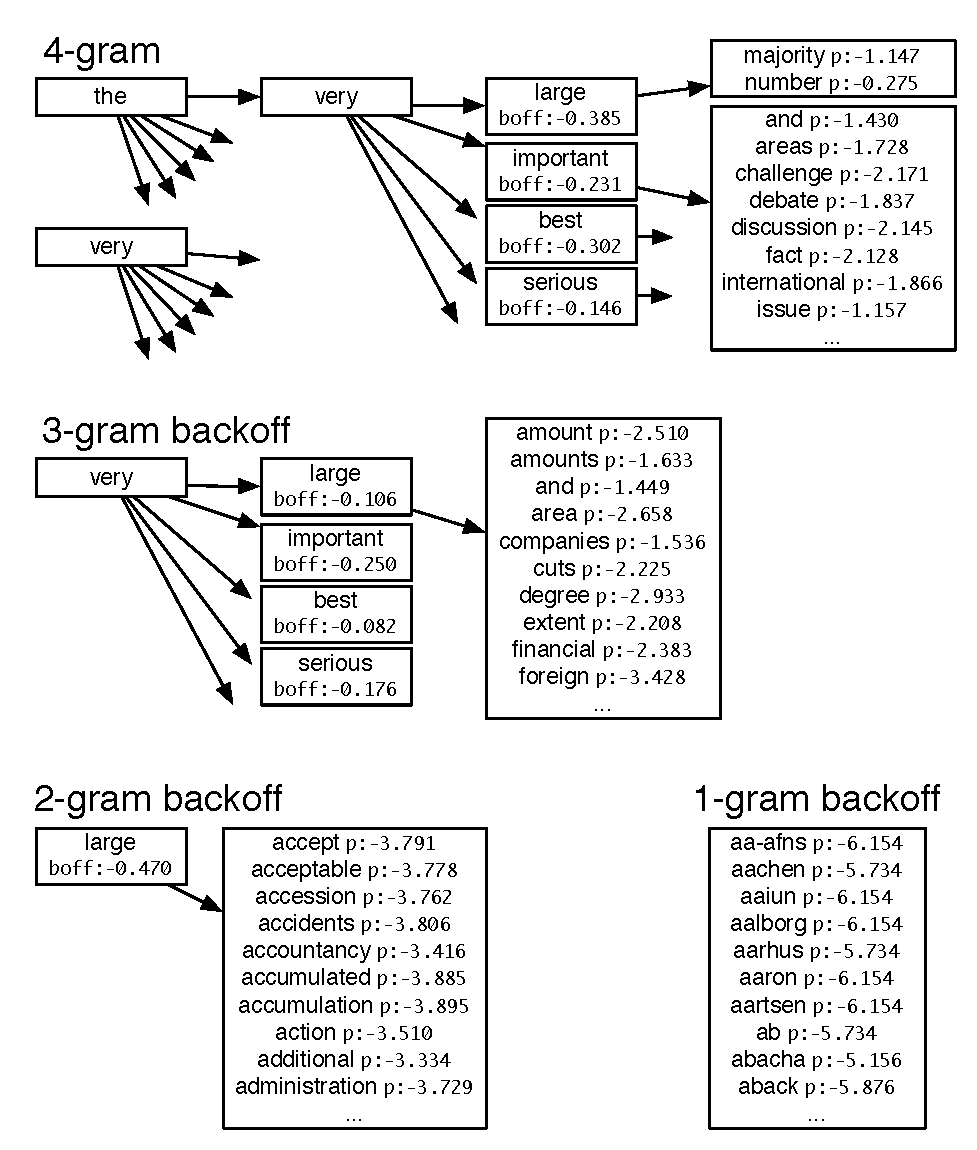
\includegraphics[scale=0.71]{lm-trie.pdf}
&
\vspace{-120mm}
\begin{itemize}
\item Need to store probabilities for
\begin{itemize}
\item \example{the very large majority}
\item \example{the very language number}
\end{itemize}
\item Both share history \example{the very large}
\item[$\rightarrow$] no need to store history twice
\item[$\rightarrow$] Trie
\end{itemize}
\end{tabular}

%%%%%%%%%%%%%%%%%%%%%%%%%%%%%%%%%%%%%%%%%%%%%%%%%%%%%%%%%%%%%%%%%%%%%%%%%%%%

\slide{Fewer Bits to Store Probabilities}
\vspace{20mm}
\begin{itemize}
\item Index for words
\begin{itemize}
\item two bytes allow a vocabulary of $2^{16}=65,536$ words, typically more needed
\item Huffman coding to use fewer bits for frequent words.
\end{itemize}
\item Probabilities
\begin{itemize}
\item typically stored in log format as floats (4 or 8 bytes)
\item quantization of probabilities to use even less memory, maybe just 4-8 bits
\end{itemize}
\end{itemize}

%%%%%%%%%%%%%%%%%%%%%%%%%%%%%%%%%%%%%%%%%%%%%%%%%%%%%%%%%%%%%%%%%%%%%%%%%%%%

\slide{Reducing Vocabulary Size}
\vspace{5mm}
\begin{itemize}
\item For instance: each number is treated as a separate token
\item Replace them with a number token \example{\sc num}
\begin{itemize}
\item but: we want our language model to prefer
\vspace{-5mm}
\maths{\begin{equation*}
p_\text{\sc lm}(\text{\example{I pay 950.00 in May 2007}}) > p_\text{\sc lm}(\text{\example{I pay 2007 in May 950.00}})
\end{equation*}}
\vspace{-12mm}
\item not possible with number token
\vspace{-5mm}
\maths{\begin{equation*}
p_\text{\sc lm}(\text{\example{I pay {\sc num} in May {\sc num}}}) = p_\text{\sc lm}(\text{\example{I pay {\sc num} in May {\sc num}}})
\end{equation*}}
\vspace{-17mm}
\end{itemize}
\item Replace each digit (with unique symbol, e.g., \example{@} or \example{5}), retain some distinctions
\vspace{-5mm}
\maths{\begin{equation*}
p_\text{\sc lm}(\text{\example{I pay 555.55 in May 5555}}) > p_\text{\sc lm}(\text{\example{I pay 5555 in May 555.55}})\vspace{-12mm}
\end{equation*}}
\end{itemize}

%%%%%%%%%%%%%%%%%%%%%%%%%%%%%%%%%%%%%%%%%%%%%%%%%%%%%%%%%%%%%%%%%%%%%%%%%%%%

\slide{Filtering Irrelevant N-Grams}
\begin{itemize}
\item We use language model in decoding
\begin{itemize}
\item we only produce English words in translation options
\item filter language model down to n-grams containing only those words
\end{itemize}
\vspace{-3mm}
\item Ratio of 5-grams needed to all 5-grams (by sentence length):
\vspace{-6mm}
\begin{center}
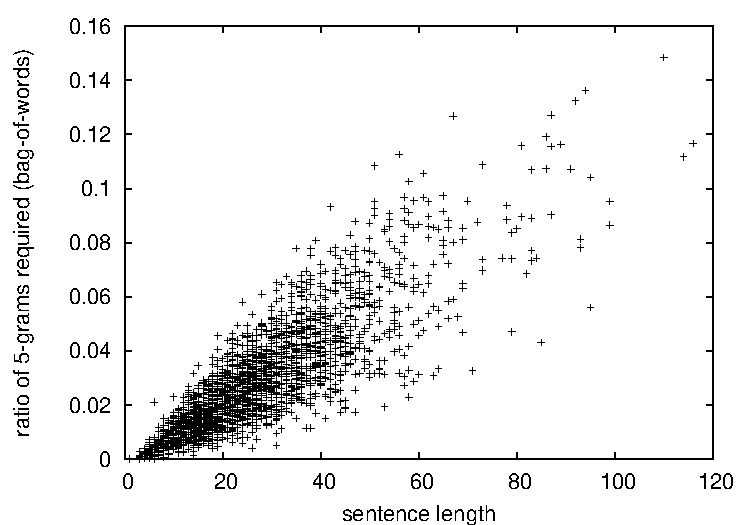
\includegraphics[scale=1]{l-s5.pdf}
\end{center} \vspace{-3mm}
\end{itemize}

%%%%%%%%%%%%%%%%%%%%%%%%%%%%%%%%%%%%%%%%%%%%%%%%%%%%%%%%%%%%%%%%%%%%%%%%%%%%

\slide{Summary}
\begin{itemize}
\item Language models: {\em How likely is a string of English words good English?}
\vspace{-3mm}
\item N-gram models (Markov assumption)
\vspace{-3mm}
\item Perplexity
\vspace{-3mm}
\item Count smoothing
\vspace{-3mm}
\begin{itemize}
\item add-one, add-$\alpha$
\item deleted estimation
\item Good Turing
\end{itemize}
\vspace{-3mm}
\item Interpolation and backoff
\vspace{-3mm}
\begin{itemize}
\item Good Turing
\item Witten-Bell
\item Kneser-Ney
\end{itemize}
\vspace{-3mm}
\item Managing the size of the model
\end{itemize}

%%%%%%%%%%%%%%%%%%%%%%%%%%%%%%%%%%%%%%%%%%%%%%%%%%%%%%%%%%%%%%%%%%%%%%%%%%%%

\end{document}
